\documentclass{article}\usepackage[]{graphicx}\usepackage[]{color}
%% maxwidth is the original width if it is less than linewidth
%% otherwise use linewidth (to make sure the graphics do not exceed the margin)
\makeatletter
\def\maxwidth{ %
  \ifdim\Gin@nat@width>\linewidth
    \linewidth
  \else
    \Gin@nat@width
  \fi
}
\makeatother

\definecolor{fgcolor}{rgb}{0.345, 0.345, 0.345}
\newcommand{\hlnum}[1]{\textcolor[rgb]{0.686,0.059,0.569}{#1}}%
\newcommand{\hlstr}[1]{\textcolor[rgb]{0.192,0.494,0.8}{#1}}%
\newcommand{\hlcom}[1]{\textcolor[rgb]{0.678,0.584,0.686}{\textit{#1}}}%
\newcommand{\hlopt}[1]{\textcolor[rgb]{0,0,0}{#1}}%
\newcommand{\hlstd}[1]{\textcolor[rgb]{0.345,0.345,0.345}{#1}}%
\newcommand{\hlkwa}[1]{\textcolor[rgb]{0.161,0.373,0.58}{\textbf{#1}}}%
\newcommand{\hlkwb}[1]{\textcolor[rgb]{0.69,0.353,0.396}{#1}}%
\newcommand{\hlkwc}[1]{\textcolor[rgb]{0.333,0.667,0.333}{#1}}%
\newcommand{\hlkwd}[1]{\textcolor[rgb]{0.737,0.353,0.396}{\textbf{#1}}}%
\let\hlipl\hlkwb

\usepackage{framed}
\makeatletter
\newenvironment{kframe}{%
 \def\at@end@of@kframe{}%
 \ifinner\ifhmode%
  \def\at@end@of@kframe{\end{minipage}}%
  \begin{minipage}{\columnwidth}%
 \fi\fi%
 \def\FrameCommand##1{\hskip\@totalleftmargin \hskip-\fboxsep
 \colorbox{shadecolor}{##1}\hskip-\fboxsep
     % There is no \\@totalrightmargin, so:
     \hskip-\linewidth \hskip-\@totalleftmargin \hskip\columnwidth}%
 \MakeFramed {\advance\hsize-\width
   \@totalleftmargin\z@ \linewidth\hsize
   \@setminipage}}%
 {\par\unskip\endMakeFramed%
 \at@end@of@kframe}
\makeatother

\definecolor{shadecolor}{rgb}{.97, .97, .97}
\definecolor{messagecolor}{rgb}{0, 0, 0}
\definecolor{warningcolor}{rgb}{1, 0, 1}
\definecolor{errorcolor}{rgb}{1, 0, 0}
\newenvironment{knitrout}{}{} % an empty environment to be redefined in TeX

\usepackage{alltt}

%\VignetteEngine{knitr::knitr}
%\VignetteIndexEntry{jackstraw: Statistical Inference using Latent Variables}

\usepackage{natbib}
\usepackage{graphics}
\usepackage{amsmath,bm}
\usepackage{indentfirst}
\usepackage[utf8]{inputenc}
\usepackage{hyperref}

\newcommand{\bY}{\bm{Y}}
\newcommand{\bL}{\bm{L}}
\newcommand{\bE}{\bm{E}}
\newcommand{\bB}{\bm{B}}

\newcommand{\by}{\bm{y}}
\newcommand{\bl}{\bm{l}}
\newcommand{\be}{\bm{e}}
\newcommand{\bb}{\bm{b}}





\title{jackstraw: Statistical Inference using Latent Variables}
\author{Neo Christopher Chung}
\IfFileExists{upquote.sty}{\usepackage{upquote}}{}
\begin{document}
\maketitle

\section{Introduction}

This is a vignette for the \verb@jackstraw@ package, which performs association tests between variables and estimated latent variables \cite{jackstraw}. Latent variables are unobserved and must be estimated directly from the data, using various techniques such as principal component analysis, logistic factor analysis, and others. However, treating estimated latent variables as independent variables in a conventional regression framework would results in an anti-conservative bias (i.e., artificially inflated significance). The jackstraw account for this fact that latent variables are estimated from the data and to protect association tests from an anti-conservative bias.

\section{Latent Variable Models}

Latent variables (LVs) can be seen as underlying sources of variation, that are hidden and/or undefined. In some cases, underlying sources of variation may be directly measured, such as disease status or sex, and conventional association tests (e.g., F-test) can be utilized to assess statistical significance of association between variables and such measurements. However, underlying sources of variation may be impossible to measure or poorly defined, such as cancer subtypes and population structure. For example, cancer subtypes based on histological tumor classification are highly imprecise.

When we have a high-dimensional data where a large number of variables are measured for each observation, LVs may be estimated from the data itself. For example, principal component analysis (PCA) is a popular technique to estimate LVs from a family of continuous data. After applying PCA to the observed data, one may like to identify variables associated with a set of principal components (PCs). We must be very careful when ``re-using'' PCs (or other estimated latent variables) to examine the observed data. In other words, an unadjusted association test between variables and PCs results in anti-conservative p-values. The jackstraw method adjust this over-fitting problem and produces valid association p-values.

\begin{figure}
\begin{center}
    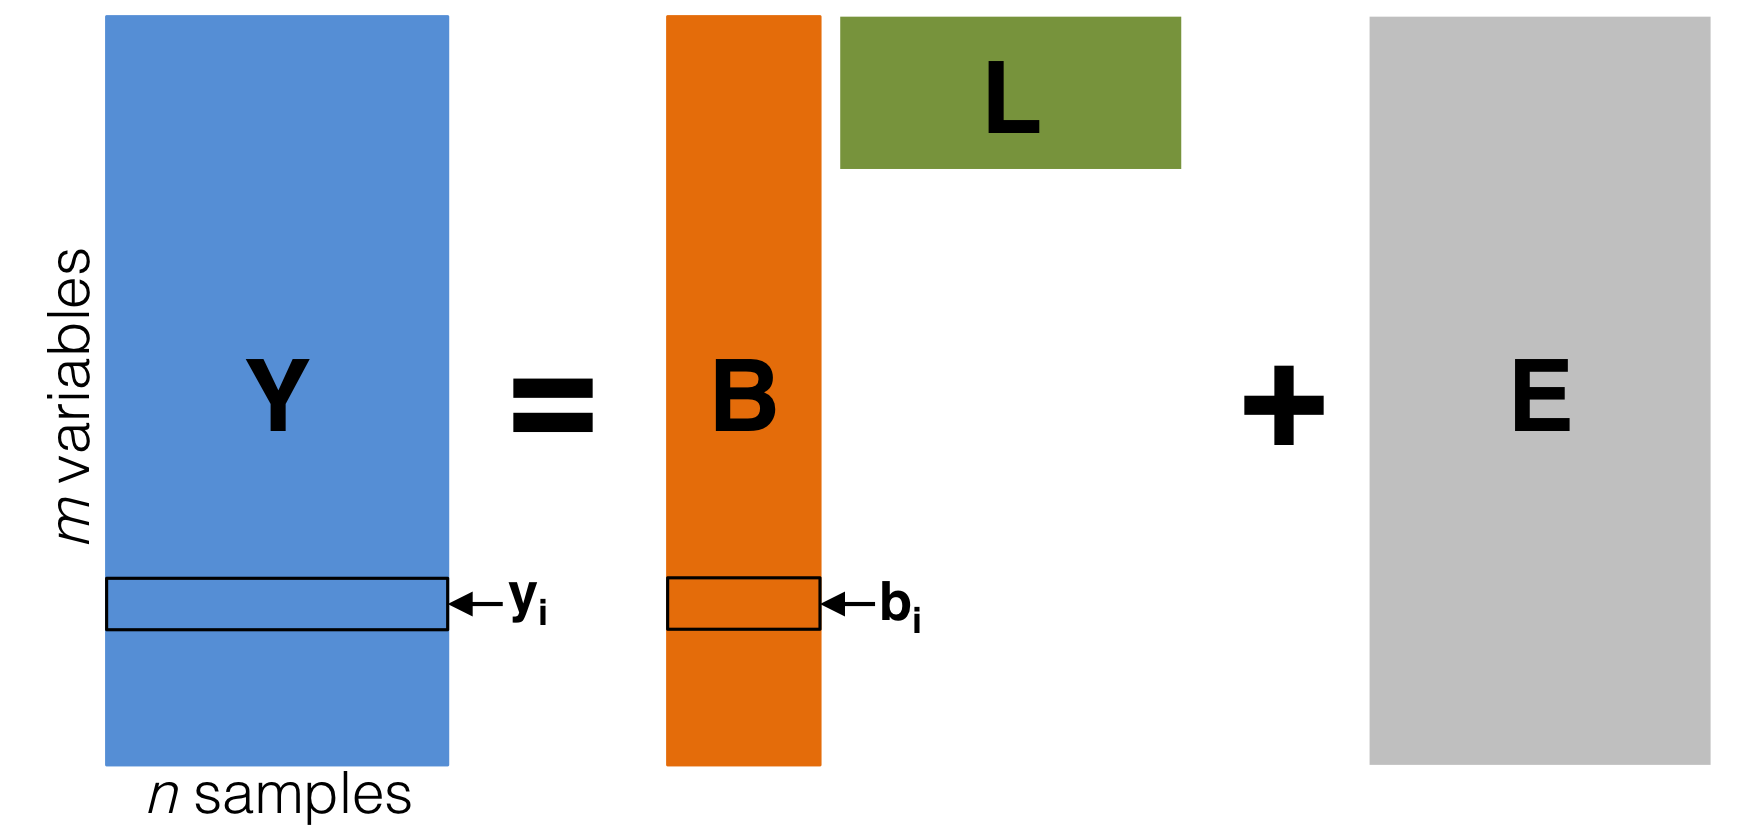
\includegraphics[width=.8\textwidth]{fixed/LatentVariableModel.png}
  \caption{{\em Diagram of the latent variable model. The latent variable basis $\bL$ is not observable, but may be estimated from $\bY$. The noise term $\bE$ is independent random variation. We are interested in performing statistical hypothesis tests on $\bb_i$ ($i=1, \ldots, m$), which quantifies the relationship between $\bL$ and $\by_i$ ($i=1, \ldots, m$). \emph{This figure is reprinted from \cite{jackstraw}}}}
\label{LVM}
\end{center}
\end{figure}

\section{Example of Continuous Data}

\subsection{Simulation of Gene Expression Data}

We simulate a simple gene expression data with $m=1000$ genes (or variables) and $n=20$ samples (or observations). The following simulation code generates a dichonomous mean shift between the first set of 10 samples and the second set of 10 samples (e.g., this may represent a case-control study). This mean shift affects $10\%$ of $m=1000$ genes:

\begin{knitrout}
\definecolor{shadecolor}{rgb}{0.969, 0.969, 0.969}\color{fgcolor}\begin{kframe}
\begin{alltt}
\hlkwd{library}\hlstd{(jackstraw)}
\hlkwd{library}\hlstd{(corpcor)}

\hlkwd{set.seed}\hlstd{(}\hlnum{1}\hlstd{)}
\hlstd{B} \hlkwb{=} \hlkwd{c}\hlstd{(}\hlkwd{runif}\hlstd{(}\hlnum{100}\hlstd{,} \hlkwc{min} \hlstd{=} \hlnum{0.1}\hlstd{,} \hlkwc{max} \hlstd{=} \hlnum{1}\hlstd{),} \hlkwd{rep}\hlstd{(}\hlnum{0}\hlstd{,} \hlnum{900}\hlstd{))}
\hlstd{L} \hlkwb{=} \hlkwd{c}\hlstd{(}\hlkwd{rep}\hlstd{(}\hlnum{1}\hlstd{,} \hlnum{10}\hlstd{),} \hlkwd{rep}\hlstd{(}\hlopt{-}\hlnum{1}\hlstd{,} \hlnum{10}\hlstd{))}
\hlstd{L} \hlkwb{=} \hlstd{L}\hlopt{/}\hlkwd{sd}\hlstd{(L)}
\hlstd{E} \hlkwb{=} \hlkwd{matrix}\hlstd{(}\hlkwd{rnorm}\hlstd{(}\hlnum{1000} \hlopt{*} \hlnum{20}\hlstd{),} \hlkwc{nrow} \hlstd{=} \hlnum{1000}\hlstd{)}
\hlstd{Y} \hlkwb{=} \hlstd{B} \hlopt \hlkwd{t}\hlstd{(L)} \hlopt{+} \hlstd{E}

\hlkwd{dim}\hlstd{(Y)}
\end{alltt}
\begin{verbatim}
## [1] 1000   20
\end{verbatim}
\begin{alltt}
\hlstd{Y[}\hlnum{1}\hlopt{:}\hlnum{5}\hlstd{,} \hlnum{1}\hlopt{:}\hlnum{5}\hlstd{]}
\end{alltt}
\begin{verbatim}
##            [,1]       [,2]        [,3]       [,4]
## [1,]  0.7284811  0.3723739  1.95390743 -0.7057011
## [2,] -0.1881271  0.6473216 -1.16625940  2.7916857
## [3,]  0.9411012 -0.4104836 -0.01000972  1.1611355
## [4,] -0.2352048  3.2953804  0.58087712  0.4482182
## [5,]  1.7074094  1.0763474 -0.64774412 -0.6600309
##             [,5]
## [1,]  0.46568781
## [2,] -0.03370393
## [3,]  0.55156033
## [4,]  0.70186429
## [5,] -0.74646792
\end{verbatim}
\end{kframe}
\end{knitrout}

\subsection{Application of the Jackstraw using PCA}

When we have a dataset, we first need to understand the type(s) of latent variables (e.g., continuous, categorical, ordinal) and to decide on a method to estimate latent variables. Let's use principal component analysis (PCA).

In practice, we have to rely on a scree plot or other graphical and statistical means to estimate $r$. One particular method is called parallel analysis from Buja and Eyuboglu (1992), which is implemented in the \verb@jackstraw@ package. The \verb@permutationPA@ function compares the observed percent variance explained (PVE) for each PC to their ``null'' counterparts computed from a randomly permuted dataset.\footnote{Determining the number of ``statistically significant'' PCs is an active area of research, and defining a number of significant PCs depends on the data structure and the context. Refer to Anderson (1963), Tracy and Widom (1996), Johnstone (2001), Leek (2010). We do not advocate the blind use of parallel analysis to obtain $\widehat{r}$.}

\begin{knitrout}
\definecolor{shadecolor}{rgb}{0.969, 0.969, 0.969}\color{fgcolor}\begin{kframe}
\begin{alltt}
\hlstd{PA} \hlkwb{=} \hlkwd{permutationPA}\hlstd{(Y,} \hlkwc{B} \hlstd{=} \hlnum{10}\hlstd{,} \hlkwc{threshold} \hlstd{=} \hlnum{0.05}\hlstd{)}
\end{alltt}


{\ttfamily\noindent\itshape\color{messagecolor}{\#\# Estimating a number of significant principal component:}}\begin{verbatim}
## 1  2  3  4  5  6  7  8  9  10
\end{verbatim}
\begin{alltt}
\hlkwd{plot}\hlstd{(PA}\hlopt{$}\hlstd{p,} \hlkwc{pch} \hlstd{=} \hlnum{20}\hlstd{,} \hlkwc{main} \hlstd{=} \hlstr{"Permutation Parallel Analysis P-values"}\hlstd{,}
    \hlkwc{ylab} \hlstd{=} \hlstr{"P-values"}\hlstd{,} \hlkwc{xlab} \hlstd{=} \hlstr{"Principal Component"}\hlstd{)}
\end{alltt}
\end{kframe}

{\centering \includegraphics[width=\maxwidth]{figure/sim_pca_PA-1} 

}



\end{knitrout}

The permutation parallel analysis suggests $r=1$, which is corroborated by the scree plot (a scatter plot of ordered PVE). Furthermore, we can visualize the first principal component (PC).

\begin{knitrout}
\definecolor{shadecolor}{rgb}{0.969, 0.969, 0.969}\color{fgcolor}\begin{kframe}
\begin{alltt}
\hlstd{svd.out} \hlkwb{=} \hlkwd{fast.svd}\hlstd{(Y)}

\hlkwd{par}\hlstd{(}\hlkwc{mfrow} \hlstd{=} \hlkwd{c}\hlstd{(}\hlnum{2}\hlstd{,} \hlnum{1}\hlstd{))}
\hlkwd{plot}\hlstd{(svd.out}\hlopt{$}\hlstd{d}\hlopt{^}\hlnum{2}\hlopt{/}\hlkwd{sum}\hlstd{(svd.out}\hlopt{$}\hlstd{d}\hlopt{^}\hlnum{2}\hlstd{),} \hlkwc{pch} \hlstd{=} \hlnum{20}\hlstd{,} \hlkwc{main} \hlstd{=} \hlstr{"The scree plot"}\hlstd{,}
    \hlkwc{xlab} \hlstd{=} \hlstr{"PC"}\hlstd{,} \hlkwc{ylab} \hlstd{=} \hlstr{"Percent Variance Explained"}\hlstd{)}
\hlkwd{plot}\hlstd{(svd.out}\hlopt{$}\hlstd{d[}\hlnum{1}\hlstd{]} \hlopt{*} \hlstd{svd.out}\hlopt{$}\hlstd{v[,} \hlnum{1}\hlstd{],} \hlkwc{pch} \hlstd{=} \hlnum{20}\hlstd{,} \hlkwc{main} \hlstd{=} \hlstr{"1st PC"}\hlstd{,}
    \hlkwc{xlab} \hlstd{=} \hlstr{"Observation"}\hlstd{,} \hlkwc{ylab} \hlstd{=} \hlstr{"Magnitude"}\hlstd{)}
\end{alltt}
\end{kframe}

{\centering \includegraphics[width=\maxwidth]{figure/sim_pca_1pc-1} 

}



\end{knitrout}

We are now ready to apply the jackstraw to our data, in order to assess statistical significance of association between variables and the first PC:

\begin{knitrout}
\definecolor{shadecolor}{rgb}{0.969, 0.969, 0.969}\color{fgcolor}\begin{kframe}
\begin{alltt}
\hlstd{js.pca} \hlkwb{=} \hlkwd{jackstraw_pca}\hlstd{(Y,} \hlkwc{r} \hlstd{=} \hlnum{1}\hlstd{,} \hlkwc{s} \hlstd{=} \hlnum{100}\hlstd{,} \hlkwc{B} \hlstd{=} \hlnum{100}\hlstd{,}
    \hlkwc{verbose} \hlstd{=} \hlnum{FALSE}\hlstd{)}

\hlkwd{hist}\hlstd{(js.pca}\hlopt{$}\hlstd{p.value,} \hlnum{10}\hlstd{,} \hlkwc{col} \hlstd{=} \hlstr{"black"}\hlstd{)}
\end{alltt}
\end{kframe}

{\centering \includegraphics[width=\maxwidth]{figure/sim_pca_jackstraw-1} 

}



\end{knitrout}

By setting \verb@method="PCA"@, the jackstraw uses a corresponding method to estimate latent variables. In this instance, this wrapper function passes along all the arguments to \verb@jackstraw.PCA@ to perform association tests between variables and principal components.

Since the data was simulated, we can visualize the ``null'' p-values for the truly null variables and the ``alternative'' p-values for the truly alternative variables. Note that the null p-values is approximating the uniform distribution between 0 and 1:

\begin{knitrout}
\definecolor{shadecolor}{rgb}{0.969, 0.969, 0.969}\color{fgcolor}\begin{kframe}
\begin{alltt}
\hlkwd{par}\hlstd{(}\hlkwc{mfrow} \hlstd{=} \hlkwd{c}\hlstd{(}\hlnum{1}\hlstd{,} \hlnum{2}\hlstd{))}
\hlkwd{hist}\hlstd{(js.pca}\hlopt{$}\hlstd{p.value[}\hlnum{1}\hlopt{:}\hlnum{100}\hlstd{],} \hlnum{10}\hlstd{,} \hlkwc{col} \hlstd{=} \hlstr{"black"}\hlstd{,} \hlkwc{main} \hlstd{=} \hlstr{"Alternative P-values"}\hlstd{)}
\hlkwd{hist}\hlstd{(js.pca}\hlopt{$}\hlstd{p.value[}\hlnum{101}\hlopt{:}\hlnum{1000}\hlstd{],} \hlnum{10}\hlstd{,} \hlkwc{col} \hlstd{=} \hlstr{"black"}\hlstd{,} \hlkwc{main} \hlstd{=} \hlstr{"Null P-values"}\hlstd{)}
\end{alltt}
\end{kframe}

{\centering \includegraphics[width=\maxwidth]{figure/sim_pca_pvalues-1} 

}



\end{knitrout}

\section{Example of Categorical Data}

\subsection{Simulation of Genotype Data}

We simulate a genotype matrix with $m=5000$ loci (or variables) and $n=100$ people (or observations). And a population structure was generated to affect only among $50\%$ of loci. This is parametized by $\pi_0=.5$. In other words, $50\%$ of loci are independent of population structure:

\begin{knitrout}
\definecolor{shadecolor}{rgb}{0.969, 0.969, 0.969}\color{fgcolor}\begin{kframe}
\begin{alltt}
\hlkwd{library}\hlstd{(jackstraw)}
\hlkwd{library}\hlstd{(lfa)}

\hlkwd{set.seed}\hlstd{(}\hlnum{2}\hlstd{)}
\hlstd{m} \hlkwb{=} \hlnum{5000}
\hlstd{n} \hlkwb{=} \hlnum{100}
\hlstd{pi0} \hlkwb{=} \hlnum{0.5}
\hlstd{m0} \hlkwb{=} \hlkwd{round}\hlstd{(m} \hlopt{*} \hlstd{pi0)}
\hlstd{m1} \hlkwb{=} \hlstd{m} \hlopt{-} \hlkwd{round}\hlstd{(m} \hlopt{*} \hlstd{pi0)}
\hlstd{B} \hlkwb{=} \hlkwd{matrix}\hlstd{(}\hlnum{0}\hlstd{,} \hlkwc{nrow} \hlstd{= m,} \hlkwc{ncol} \hlstd{=} \hlnum{1}\hlstd{)}
\hlstd{B[}\hlnum{1}\hlopt{:}\hlstd{m1, ]} \hlkwb{=} \hlkwd{matrix}\hlstd{(}\hlkwd{runif}\hlstd{(m1} \hlopt{*} \hlstd{n,} \hlkwc{min} \hlstd{=} \hlopt{-}\hlnum{0.5}\hlstd{,} \hlkwc{max} \hlstd{=} \hlnum{0.5}\hlstd{),}
    \hlkwc{nrow} \hlstd{= m1,} \hlkwc{ncol} \hlstd{=} \hlnum{1}\hlstd{)}
\hlstd{L} \hlkwb{=} \hlkwd{matrix}\hlstd{(}\hlkwd{rnorm}\hlstd{(n),} \hlkwc{nrow} \hlstd{=} \hlnum{1}\hlstd{,} \hlkwc{ncol} \hlstd{= n)}
\hlstd{BL} \hlkwb{=} \hlstd{B} \hlopt \hlstd{L}
\hlstd{prob} \hlkwb{=} \hlkwd{exp}\hlstd{(BL)}\hlopt{/}\hlstd{(}\hlnum{1} \hlopt{+} \hlkwd{exp}\hlstd{(BL))}

\hlstd{dat} \hlkwb{=} \hlkwd{list}\hlstd{(}\hlkwc{Y} \hlstd{=} \hlkwd{matrix}\hlstd{(}\hlkwd{rbinom}\hlstd{(m} \hlopt{*} \hlstd{n,} \hlnum{2}\hlstd{,} \hlkwd{as.numeric}\hlstd{(prob)),}
    \hlstd{m, n),} \hlkwc{H} \hlstd{=} \hlkwd{c}\hlstd{(}\hlkwd{rep}\hlstd{(}\hlnum{1}\hlstd{, m1),} \hlkwd{rep}\hlstd{(}\hlnum{0}\hlstd{, m0)))}

\hlkwd{dim}\hlstd{(dat}\hlopt{$}\hlstd{Y)}
\end{alltt}
\begin{verbatim}
## [1] 5000  100
\end{verbatim}
\begin{alltt}
\hlstd{dat}\hlopt{$}\hlstd{Y[}\hlnum{1}\hlopt{:}\hlnum{5}\hlstd{,} \hlnum{1}\hlopt{:}\hlnum{5}\hlstd{]}
\end{alltt}
\begin{verbatim}
##      [,1] [,2] [,3] [,4] [,5]
## [1,]    1    0    1    0    0
## [2,]    1    0    1    2    2
## [3,]    0    0    2    2    2
## [4,]    2    0    0    0    1
## [5,]    1    0    1    2    2
\end{verbatim}
\end{kframe}
\end{knitrout}

The output includes the genotype matrix \verb@dat$Y@, the status of hypothesis \verb@dat$H@, and the true probability from which the data is simulated \verb@dat$prob@. See that the simulated genotype matrix is encoded in $0,1,2$.

\subsection{Application of the Jackstraw using LFA}

With a genotype matrix, we can use the Logistic Factor Analysis from \cite{lfa}. We are interested in identifying loci which are truly associated with an underlying population structure (which we must directly estimated from the genotype matrix). LFA estimates this underlying population structure with ``logistic factors (LFs)'' and we will carry out association tests between loci and LFs.

\begin{knitrout}
\definecolor{shadecolor}{rgb}{0.969, 0.969, 0.969}\color{fgcolor}\begin{kframe}
\begin{alltt}
\hlstd{js.lfa} \hlkwb{=} \hlkwd{jackstraw_lfa}\hlstd{(dat}\hlopt{$}\hlstd{Y,} \hlkwc{r} \hlstd{=} \hlnum{2}\hlstd{,} \hlkwc{FUN} \hlstd{=} \hlkwa{function}\hlstd{(}\hlkwc{x}\hlstd{)} \hlkwd{lfa.corpcor}\hlstd{(x,}
    \hlnum{2}\hlstd{)[, ,} \hlkwc{drop} \hlstd{=} \hlnum{FALSE}\hlstd{],} \hlkwc{s} \hlstd{=} \hlnum{200}\hlstd{,} \hlkwc{B} \hlstd{=} \hlnum{10}\hlstd{,} \hlkwc{devR} \hlstd{=} \hlnum{TRUE}\hlstd{)}
\end{alltt}
\begin{verbatim}
## 
## Computating null statistics (10 total iterations): 1  2  3  4  5  6  7  8  9  10
\end{verbatim}
\begin{alltt}
\hlkwd{hist}\hlstd{(js.lfa}\hlopt{$}\hlstd{p.value,} \hlnum{10}\hlstd{,} \hlkwc{col} \hlstd{=} \hlstr{"black"}\hlstd{)}
\end{alltt}
\end{kframe}

{\centering \includegraphics[width=\maxwidth]{figure/sim_lfa_jackstraw-1} 

}



\end{knitrout}

Since the data was simulated, we can look at p-values according to their true status. In this case, we see that the null p-values are again approximately distributed uniformly between 0 and 1:

\begin{knitrout}
\definecolor{shadecolor}{rgb}{0.969, 0.969, 0.969}\color{fgcolor}\begin{kframe}
\begin{alltt}
\hlkwd{par}\hlstd{(}\hlkwc{mfrow} \hlstd{=} \hlkwd{c}\hlstd{(}\hlnum{1}\hlstd{,} \hlnum{2}\hlstd{))}
\hlkwd{hist}\hlstd{(js.lfa}\hlopt{$}\hlstd{p.value[}\hlkwd{which}\hlstd{(dat}\hlopt{$}\hlstd{H} \hlopt{==} \hlnum{1}\hlstd{)],} \hlnum{10}\hlstd{,} \hlkwc{col} \hlstd{=} \hlstr{"black"}\hlstd{,}
    \hlkwc{main} \hlstd{=} \hlstr{"Alternative P-values"}\hlstd{)}
\hlkwd{hist}\hlstd{(js.lfa}\hlopt{$}\hlstd{p.value[}\hlkwd{which}\hlstd{(dat}\hlopt{$}\hlstd{H} \hlopt{==} \hlnum{0}\hlstd{)],} \hlnum{10}\hlstd{,} \hlkwc{col} \hlstd{=} \hlstr{"black"}\hlstd{,}
    \hlkwc{main} \hlstd{=} \hlstr{"Null P-values"}\hlstd{)}
\end{alltt}
\end{kframe}

{\centering \includegraphics[width=\maxwidth]{figure/sim_lfa_pvalues-1} 

}



\end{knitrout}

\clearpage

\bibliographystyle{plain}
\bibliography{refs}

\end{document}
